Im vorherigen Kapitel wurden die Ergebnisse für ein episodales Problem vorgestellt. Dieses Kapitel präsentiert nun die Resultate für das kontinuierliche Lernszenario \textit{AntGame}, bei dem kein Terminalzustand vorhanden ist und somit keine Episoden erzeugt werden können. Folglich werden alle Experimente mit einem \textit{Temporal-Difference} Algorithmus, genauer dem \textit{Q-Learning}, durchgeführt. 
\par 
Zunächst werden die Auswirkungen von verschiedenen Kombinationen von Diskontierungsfaktor und Lernrate gezeigt. Anschließend wird geklärt, ob \textit{Q-Learning} in der Lage ist, optimales Verhalten zu erlernen, d.h. direkte Wege zu laufen und so effizient wie möglich Futter zu sammeln.


\subsubsection{Auswirkung Diskontierungsfaktor und Lernrate}
Im Vergleich zu den MC-Methoden haben zwei weitere Parameter Einfluss auf das Lernen bei dem \textit{Q-Learning}, genauer gesagt den TD-Methoden als Ganzes. Zum einen der Diskontierungsfaktor $\gamma$, der bei MC-Methoden in der Theorie den Wert 1 hat und somit nicht explizit erwähnt wird. Die Auswirkungen von $\gamma$ wurden in Kapitel \ref{sec:Gewinne} erläutert und werden in diesem Unterabschnitt praktisch untersucht. Zum anderen die Lernrate $\alpha$, die in Kapitel \ref{sec:TD} erwähnt worden ist und eine Gewichtung darstellt für die Anpassung alter Werte von $q(s,a)$ durch neue Schätzungen.

\subsubsection*{Methodik}
Für die Untersuchungen für diesen Unterabschnitt wurde die detaillierte Belohnungsfunktion $B_3$ verwendet, jedoch mit einer kleinen Modifikation. Statt einer Belohnung von +1 für das erfolgreiche Ablegen von Futter in das Nest der Ameise wurde eine Belohnung von +40 verteilt, um eine größere Differenz zwischen den durchschnittlichen Belohnungen pro Zeitstempel im Verlauf zu erzeugen.
\par 
Alle Experimente wurden mit dem Explorationsfaktor $\epsilon = 0.15$ durchgeführt.
\par 
Die Werte für die durchschnittliche Belohnung pro Zeitstempel ergeben sich aus den Durchschnitten für jeweils 1000 Zeitstempel.

\subsubsection*{Kombinationen Diskontierungsfaktor und Lernrate}
Folgende Untersuchungen sollen explizit keine Aussage über die Fähigkeit für das Erreichen des optimalen Verhaltens treffen, sondern zeigen, wie sich Diskontierungsfaktor und Lernrate auf das Konvergenzverhalten des \textit{Q-Learnings} an sich auswirken.
\par 
Wie eingangs erwähnt, gibt die Lernrate $\alpha$ an, wie schnell neue Gegebenheiten bzw. Schätzungen vorhandene Aktions-Nutzen verändern. Höhere Lernrate sorgt somit dafür, dass der Algorithmus sich rascher an neue Eigenschaften der Umwelt anpasst und alte Lernfortschritte überschreibt. Da die Umwelt des \textit{AntGames} stationär ist und sich im Verlauf der Interaktion nicht ändert, ist anzunehmen, dass eine sehr hohe Lernrate zu schnellerer Konvergenz führt.
\par 
Interessant ist zudem die Einwirkung des Diskontierungsfaktors $\gamma$. Mit Worten umschrieben sagt dieser aus, wie \glqq weitsichtig\grqq{} ein Agent handeln soll. Im Fall des \textit{AntGames} bekommt der Agent erst eine positive Belohnung, wenn er Futter aufsammelt und es auf das Nest ablegt. In der Zwischenzeit erhält er ausschließlich negative Belohnungen und muss somit die Fähigkeit haben, zu wissen, dass in der Zukunft, unter bestimmten Entscheidungsverhalten, eine positive Belohnung auf ihn wartet. 
\par 
Der erste Diskontierungsfaktor, der getestet wird, ist $0.5$:
\begin{figure}[H]
    \centering
    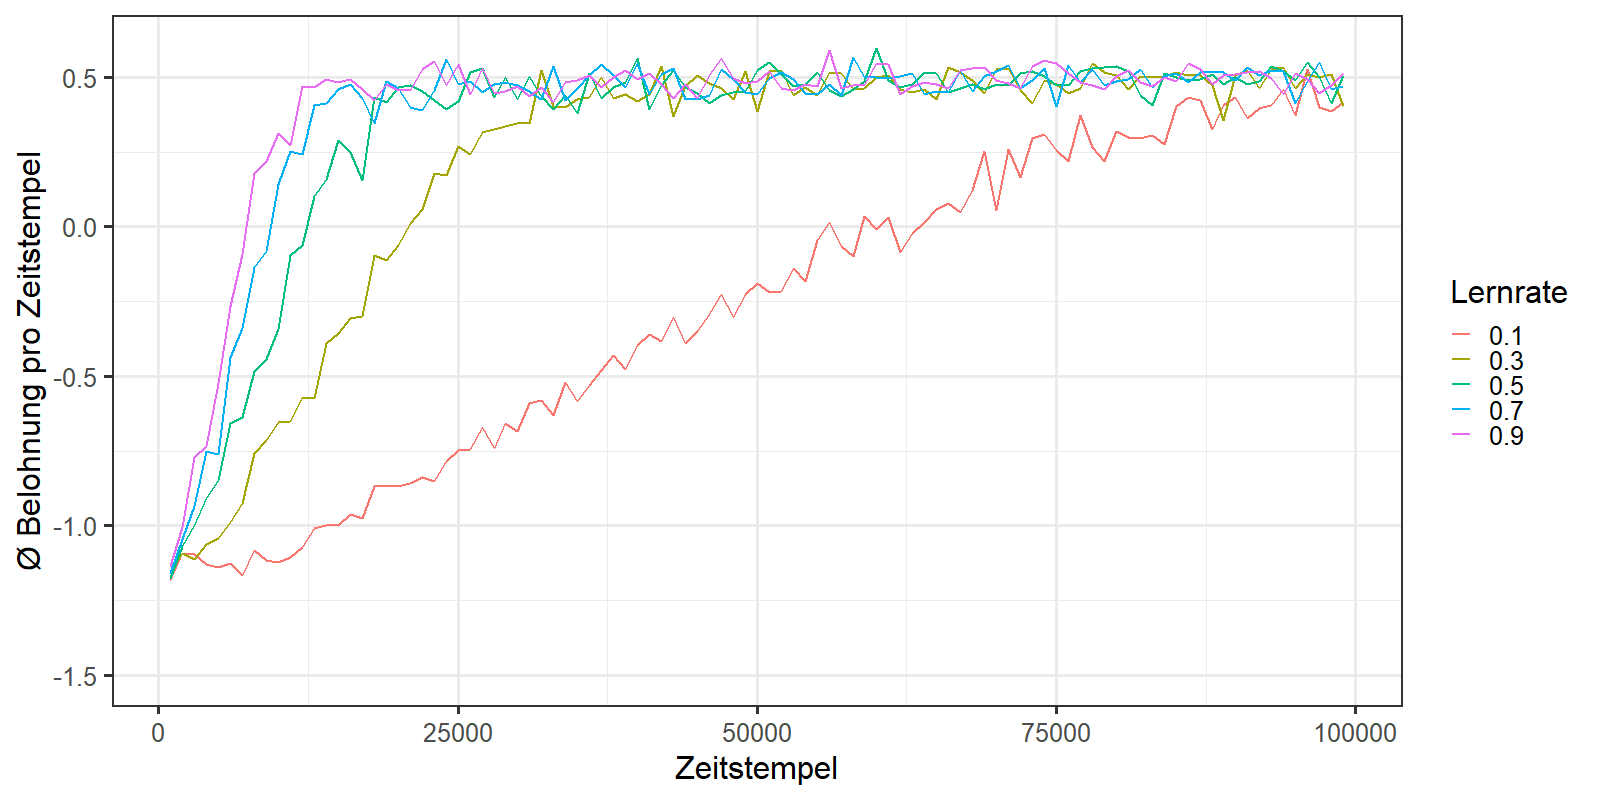
\includegraphics[width=\textwidth]{images/antGameAnalysis05DiscA}
    \captionof{figure}{Durchschnittliche Belohnung pro Zeitstempel bei $\gamma = 0.5$ und $\epsilon = 0.15$}
    \label{fig:test1}
\end{figure}
Bezogen auf die Lernrate $\alpha$ konnte die ursprüngliche Annahme bestätigt werden. Alle Durchläufe konvergieren zwar auf eine durchschnittliche Belohnung pro Zeitstempel von circa 0.5, jedoch wird diese Konvergenz mit steigender Lernrate schneller erreicht. Eine Lernrate von 0.9 benötigt rund 12500 Zeitstempel, wohingegen eine Lernrate von 0.1 über 100000 Zeitstempel benötigt, um zu konvergieren. Durch ein weiteres Experiment, welches nicht Teil der Abbildung ist, konnte zudem bewiesen werden, dass sogar eine Lernrate von $\alpha = 1$ praktikabel für dieses stationäre Problemszenario ist und am schnellsten konvergiert.
\par 
Das zweite Experiment wurde mit einem höheren Diskontierungsfaktor von $\gamma=0.9$ durchgeführt:
\begin{figure}[H]
    \centering
    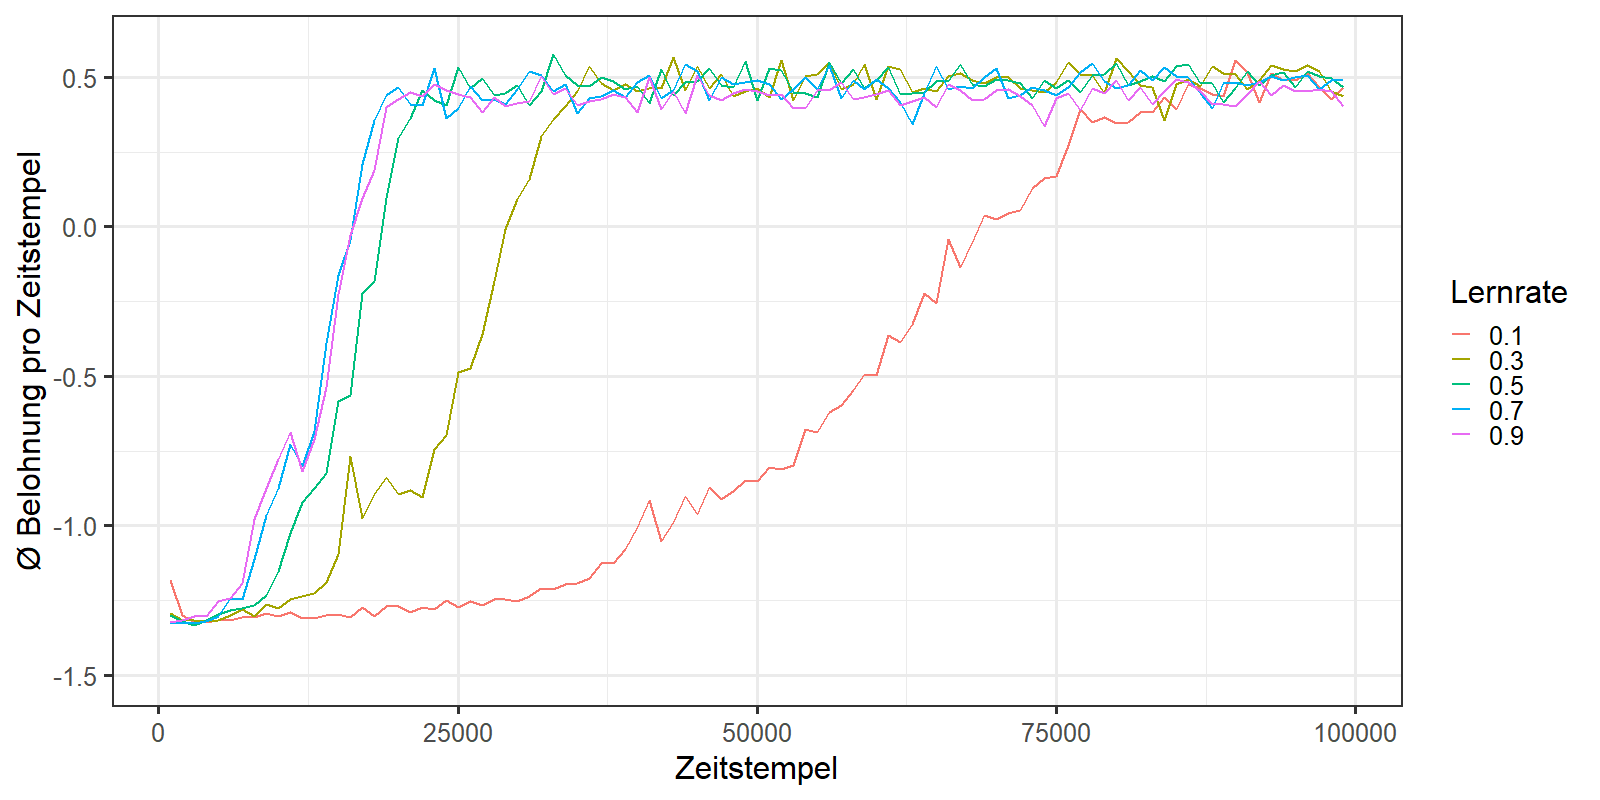
\includegraphics[width=\textwidth]{images/antGameAnalysis09DiscA}
    \captionof{figure}{Durchschnittliche Belohnung pro Zeitstempel bei $\gamma = 0.9$ und $\epsilon = 0.15$}
    \label{fig:gamma09}
\end{figure}
Zu erkennen ist, dass sämtliche Durchgänge zu Beginn des Lernens eine deutlich schlechtere durchschnittliche Belohnung pro Zeitstempel erhalten. Bei dem vorherigen Experiment in Abbildung \ref{fig:gamma09}, erleben alle Durchläufe (mit Ausnahme des $\alpha = 0.9$ Durchlaufs) einen starken Anstieg direkt zu Beginn des Lernprozesses. Durch die Erhöhung des Diskontierungsfaktors $\gamma$ auf einen Wert von 0.9 agiert der Agent zu weitsichtig im Bezug auf dieses Problem. Der Agent betrachtet nicht den erwarteten Gewinn bis zu dem Ablegen einer Futtereinheit und der daraus resultierenden positiven Belohnung, sondern weit darüber hinaus. Dies hat zur Folge, dass erfolgreiche Entscheidungssequenzen zunächst schlechter erscheinen, weil negative Belohnungen nach dem Ablegen zu optimalen Entscheidungen der Vergangenheit und deren erwarteter Gewinn hinzuaddiert werden. Anders ausgedrückt lernt und bewertet der Agent nicht Entscheidungsreihenfolgen, um eine Futterquelle aufzunehmen und auf dem Nest abzulegen, sondern Reihenfolgen, die beispielsweise 10 Futtereinheiten auf optimalen Weg sammeln. Dadurch erhöht sich der Aufwand der Exploration und der Iterationen bis zu einer korrekten Bewertung der Aktions-Nutzen.
\par 
Diese Schlussfolgerung lässt sich zudem sehr gut durch einen noch höheren Wert für $\gamma$ überprüfen. Wie in Kapitel \ref{sec:Gewinne} erläutert, darf $\gamma$ nicht den Wert 1 für kontinuierliche Probleme annehmen, da sonst der Gewinn, also die Summe der erhaltenen Belohnungen unendlich ist. Erlaubt ist jedoch ein Wert sehr nah an 1, wie z.B. 0.99:
\begin{figure}[H]
    \centering
    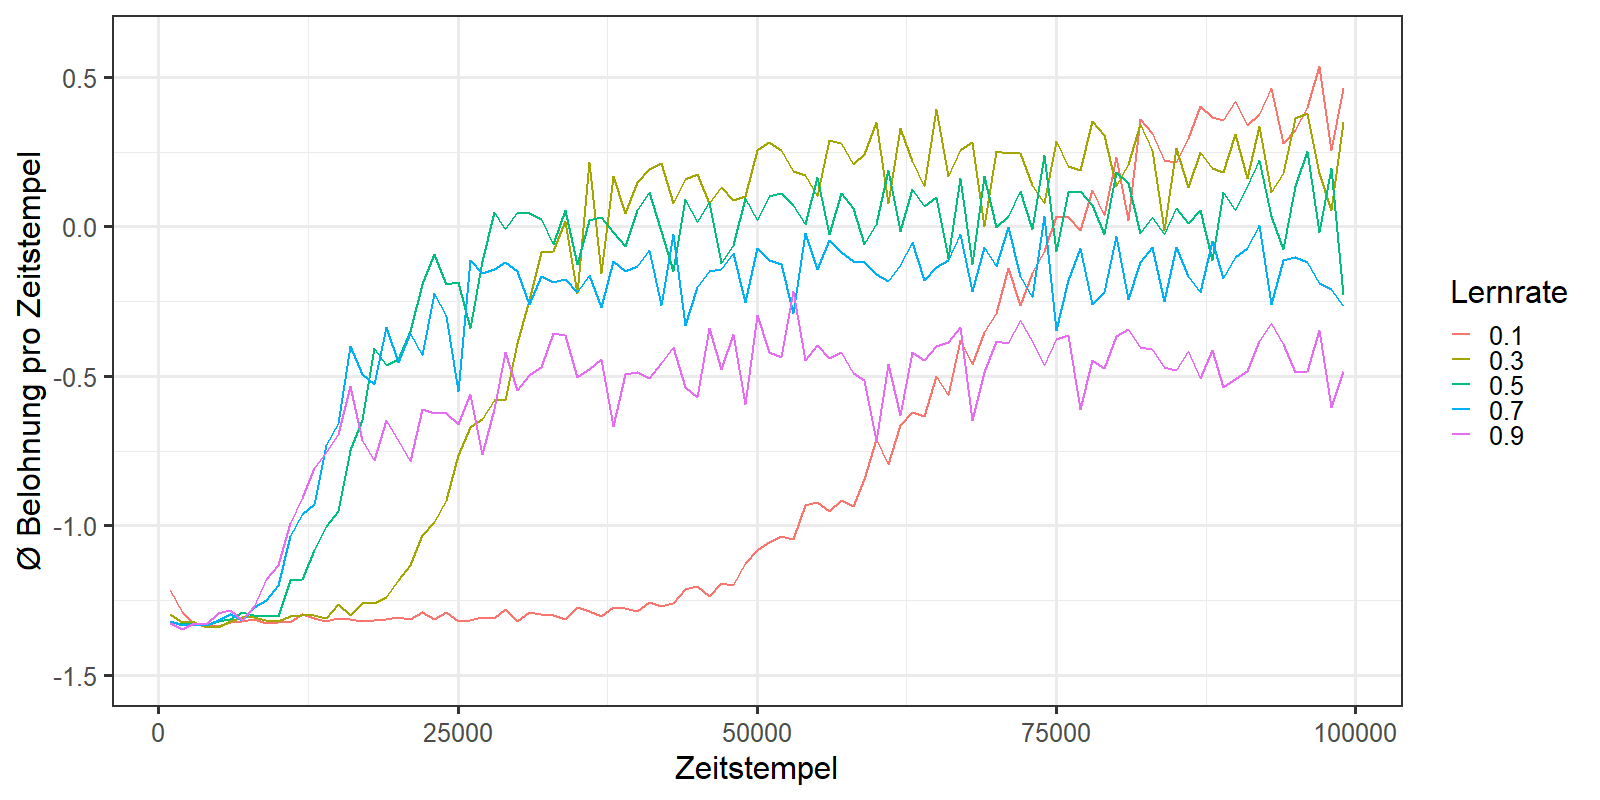
\includegraphics[width=\textwidth]{images/antGameAnalysis099DiscA}
    \captionof{figure}{Durchschnittliche Belohnung pro Zeitstempel bei $\gamma = 0.99$ und $\epsilon = 0.15$}
    \label{fig:test1}
\end{figure}
Eine erneute Abschwächung der durchschnittlich erhaltenen Belohnung pro Zeitstempel ist festzustellen, vor allem in Kombinationen mit einer sehr niedrigen Lernrate von $0.1$. Ein positiver Lerneffekt kann unter diesen Bedingungen erst nach circa 48000 Zeitstempeln bemerkt werden. Auch die restlichen Durchläufe zeigen eine deutlich schlechtere Performance und große Schwankungen im Vergleich zu den beiden vorigen Experimenten. Keine Konfiguration schafft es innerhalb von 100000 Zeitstempeln auf den durchschnittlichen Belohnungswert von 0.5 zu konvergieren. 
\par 
Es erscheint zudem, als ob höhere Lernraten zu einem niedrigeren lokalen Maximum führen. Lokal deshalb, weil alle Konfiguration letztendlich zu dem gleichen Ergebnis für die durchschnittlichen Belohnungen konvergieren wie in den beiden Experimenten zuvor, jedoch erst nach Millionen von Zeitstempeln. Erklären lassen sich die unterschiedlichen Maxima damit, dass hohe Lernraten dafür sorgen, dass schneller vermeintlich optimale Entscheidungssequenzen gelernt werden, die Futter zwar aufsammeln, aber nicht auf dem direkten Weg. Je geringer die Lernrate, desto mehr mögliche Reihenfolgen bilden den Durchschnitt für den erwarteten Gewinn, also auch mehr zufällig gewählte direkte Wege zum Futter und zurück.

\subsubsection{Optimales Verhalten}\label{sec:optimalesVerhalten}
Nachdem im vorigen Unterabschnitt alleine die Auswirkungen zweier Parameter untersucht worden sind, geht es in diesem Unterabschnitt um das Konvergenzverhalten zu dem optimalen Verhalten und der Fragestellung, ob das \textit{Q-Learning} lernt einen Wegfindungsalgorithmus zu imitieren und die Ameise optimal zu steuern, d.h. ohne Umwege zu dem Futter zu leiten, um dieses anschließend in das Nest ablegen zu können.

\subsubsection*{Methodik}
Optimales Verhalten der Ameise spiegelt sich insofern wider, das die Ameise immer die kürzeste Route wählt, keine unnötigen Aktionen ausführt und nicht gegen Hindernisse läuft. Es stellt sich zunächst die Frage, wie gemessen werden kann, ob der Agent ein solches Verhalten erzeugt. 
\par 
Der erste Schritt besteht darin, zu ermitteln, wie viele Aktionen die Ameise von dem Startfeld aus ausführen muss, um optimal zu handeln. Erscheint eine Futtereinheit direkt neben dem Startfeld, benötigt die Ameise z.B. vier Aktionen (\textit{MOVE\_LEFT, PICK\_UP, MOVE\_RIGHT, DROP\_DOWN}). Die Anzahl der benötigten Aktionen wird nun für jedes Feld berechnet:
\begin{figure}[H]
    \centering
    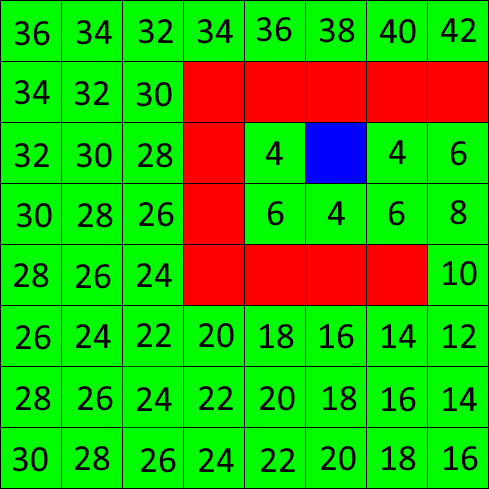
\includegraphics[width=150px]{images/NeededTimestampsFromEverywhere}
    \captionof{figure}{Minmal benötigte Aktionen für optimales Verhalten}
    \label{fig:test1}
\end{figure}
Daraufhin wird der Durchschnitt für die benötigten Aktionen bzw. Zeitstempel für ein Futter berechnet. Dieser beträgt $22.92$ Zeitstempel pro Futtereinheit. Während des Lernprozesses wird jetzt der durchschnittliche Aufwand pro Futtereinheit berechnet, indem die benötigten Zeitstempel durch 1000 geteilt werden für jeweils 1000 gesammelte Futtereinheiten. Schwankt der Durchschnitt des Agenten um den optimalen Durchschnitt, dann ist optimales Verhalten erreicht worden.
\par 
Der Explorationsparameter $\epsilon$ wurde im Laufe des Lernens verringert, um letztendlich willkürliches Verhalten zu verhindern. Gestartet wird mit einem Wert $\epsilon = 0.2$. Für jede 1000 gesammelte Futtereinheit wird dieser Wert um 0.05 verringert, bis er schließlich bei 4000 gesammelten Einheiten 0 erreicht. 
\par 
Da durch den vorigen Unterabschnitt gezeigt wurde, dass eine hohe Lernrate für dieses spezifische Problemszenario ausschließlich schnellere Konvergenzen bedeuten, wird die Lernrate $\alpha = 0.9$ gewählt.

\subsubsection*{Verhalten bei unterschiedlichen Diskontierungsfaktoren}
Dass der Diskontierungsfaktor eine entscheidende Rolle für das Konvergenzverhalten spielt, haben vor allem die Experimente des vorherigen Unterabschnitts gezeigt. Zu hohe Werte für $\gamma$ sorgen für eine deutlich langsamere Konvergenz, doch bewirkt diese auch optimales Verhalten? Kann der Agent zu \glqq kurzsichtig\grqq{} sein, wenn $\gamma$ zu niedrig gewählt wird? 
Das nachfolgende Experiment untersucht, ob unterschiedliche Diskontierungsfaktoren zu optimalen Verhalten führen oder nicht. Dabei ist das optimale Verhalten ($22.92$ Zeitstempel pro Futter) mit einer schwarz gestrichelten Linie markiert.
\begin{figure}[H]
    \centering
    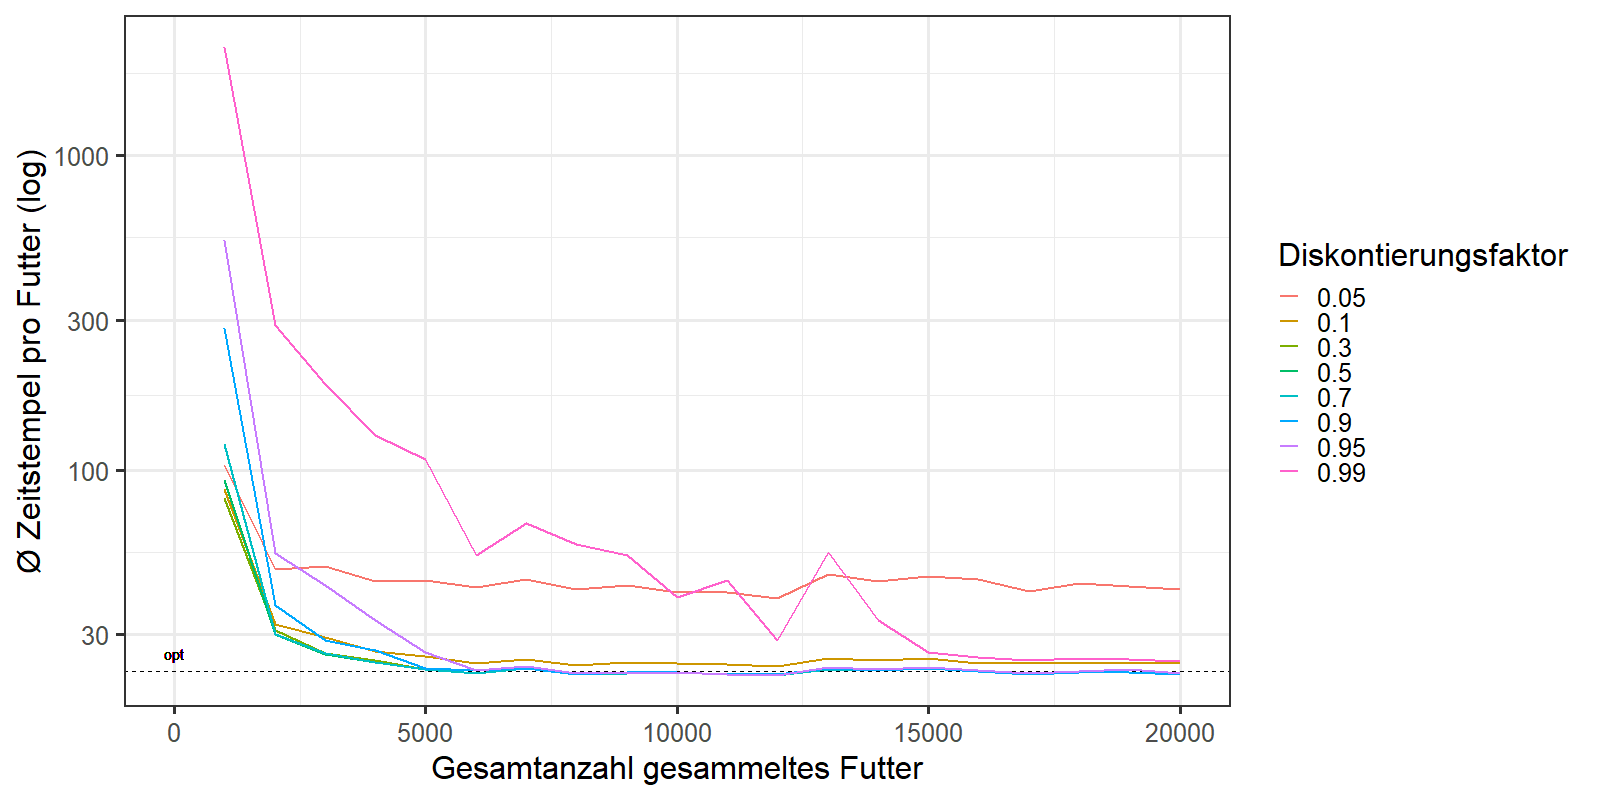
\includegraphics[width=\textwidth]{images/optDisc}
    \captionof{figure}{Optimales Verhalten bei unterschiedlichen Diskontierungsfaktoren}
    \label{fig:optDisc}
\end{figure}
Ein Diskontierungsfaktor zwischen 0.3 und 0.9 sorgt für eine Konvergenz zu optimalem Verhalten, nachdem der Explorationsparameter$\epsilon$ nach 4000 gesammelten Futtereinheit auf 0 gesetzt worden ist. Ein hoher Wert von $\gamma = 0.95$ erreicht erst nach rund 6000 Episoden optimales Verhalten, kann also noch nach dem Wegfallen der Exploration durch Anpassung der Aktions-Nutzen lernen. Auffällig ist, dass bei dem höchsten Wert für $\gamma$, 0.99, deutlich mehr Zeitstempel benötigt werden für die ersten 1000 Futtereinheit, 2205 im Vergleich zu nur 81 bei $\gamma = 0.3$. 
\par 
Die Abbildung \ref{fig:optDisc} zeigt, dass der Durchlauf mit $\gamma = 0.99$ knapp mehr durchschnittliche Zeitstempel benötigt als das optimale Verhalten. Dies gilt jedoch speziell für die gewählten Schranken für die Verringerung von $\epsilon$. Wird die letzte Senkung von 0.05 auf 0, auf eine Schranke von 20000 gesammelten Einheiten verändert, dann konvergiert auch $\gamma = 0.99$ zu optimalen Verhalten. Durch die \glqq Weitsichtigkeit\grqq{} sind die Entscheidungsreihenfolge umfangreicher und eine längere Exploration muss stattfinden, um die Gewinne für das \textit{bootstrapping} genauer zu schätzen.
\par 
Anders ist dies der Fall für die $\gamma$-Werte 0.1 und 0.05. Bei $\gamma = 0.1$ pendelt sich der Agent auf durchschnittlich 24.3 Zeitstempeln pro gesammeltes Futter ein, bei $\gamma = 0.05$ sind es circa $42$ Zeitstempel. Das entstehende Verhalten weicht folglich deutlich von dem optimalen Verhalten ab. Grund für dieses Ergebnis ist, dass der Agent in der Tat zu \glqq kurzsichtig\grqq{} geworden ist. Gespeicherte Aktions-Nutzen basieren auf geschätzten Gewinnen, deren Zusammensetzung nicht die notwendigen Belohnungen der Zukunft beinhaltet, die bei dem Ablegen des Futters in das Nest erhalten werden. Wird der Ameise nach dem Lernprozess bei ihrer Suche nach Futter zugeschaut, so ist dieser Effekt deutlich erkennbar. Erscheint Futter in der Nähe des Nestes, dann agiert die Ameise optimal und läuft die kürzesten Wege. Zu weit von dem Nest entfernt erschienendes Futter setzt jedoch lange, erlernte Entscheidungsreihenfolge über viele Zeitstempel voraus. Da diese bei zu geringem Diskontierungsfaktor allerdings nicht berücksichtigt werden, bewegt sich die Ameise zufällig auf den Feldern um das Nest hin und her, bis sie zufällig in Reichweite für das Futter gelangt, um erneut optimal zu laufen. Hat sie das Futter aufgenommen, dann wandert sie aufs Neue willkürlich umher, bis das Nest in Reichweite ist.
\par 
Die Erkenntnis, dass zu geringe Werte für $\gamma$ optimales Verhalten verhindern, im Bezug auf diese konkrete Aufgabenstellung, lässt sich zudem durch die nachfolgende Abbildung erkennen. Gezeigt werden die total benötigten Zeitstempel bei fortlaufender Sammlung von Futter.
\begin{figure}[H]
    \centering
    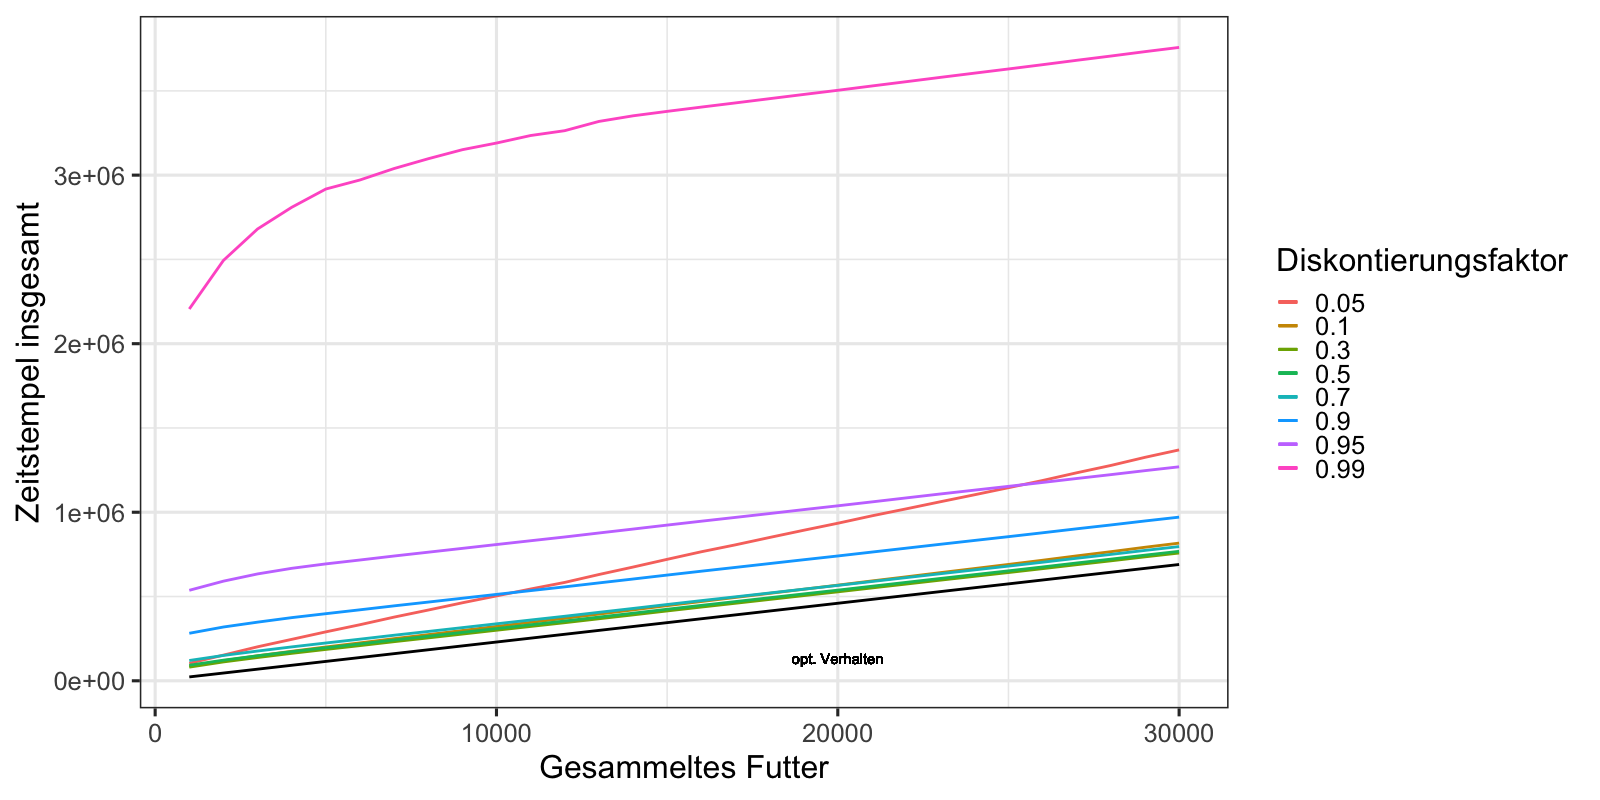
\includegraphics[width=\textwidth]{images/optDiscTotalTS}
    \captionof{figure}{Total benötigte Zeitstempel bei fortlaufender Futtersammlung}
    \label{fig:test1}
\end{figure}
Ist das optimale Verhalten gefunden, dann ist die Steigung jeder Linie gleich und entspricht $22.9$ Zeitstempel pro gesammeltem Futter. Folglich dürfte keine Linie eine andere nach erfolgreicher Konvergenz kreuzen. Dies ist jedoch bei $\gamma = 0.05$ und $\gamma = 0.1$ der Fall, da ihre Steigung $42$ respektive $24.3$ betragen.
\par 
Zusätzlich soll diese Abbildung zeigen, wie viele Zeitstempel insgesamt benötigt werden, um eine Konvergenz zu erzielen. Sind es bei $\gamma = 0.3$ 186k Zeitstempel für 5000 gesammelte Futtereinheiten, ist der Aufwand bei $\gamma = 0.99$ mit 2.9M benötigten Zeitstempeln um mehr als den Faktor 15 größer.

\subsubsection{Zusammenfassung}
Das \textit{AntGame} zeigt, dass der Diskontierungsfaktor stark von der gestellten Aufgabe abhängig ist. In der Theorie kann für kontinuierliche Probleme stets ein Wert sehr nah an 1 gewählt werden z.b. 0.99. Doch wie dargestellt, dauert der Lernprozess in diesem Fall deutlich länger (Faktor 15), als eine geeignete Größe, die auf das konkrete Problem zugeschnitten ist. Weiterhin wurde gezeigt, dass zu kleine Werte für $\gamma$ dafür sorgen, dass der Agent zu \glqq kurzsichtig\grqq{} wird und überhaupt nicht in der Lage ist, zu dem optimalen Verhalten zu konvergieren.
\par 
Größere Lernraten sorgen in allen Experimenten für eine schnellere Konvergenz. Lernraten an sich sind nützlich für sich verändernde Umwelten. Niedrige Lernraten passen die Werte der gespeicherten Nutzen dann sehr vorsichtig an die neuen Verhältnisse an. Da in dem Beispiel des AntGames jedoch eine stationäre Umwelt gegeben ist, sind höhere Lernraten genauer gesagt eine Lernrate $\alpha = 1$ zu präferieren.
\par 
Durch die gewählte Zustandsmodellierung, bei der dem Agenten die gesamte Spielfeldkonstellation bewusst ist, kann optimales Verhalten erlernt werden, unter der Bedingung, dass $\gamma >= 0.3$. Optimales Verhalten äußert sich dadurch, dass die Ameise stets auf direktem Wege zu dem Futter und zurück läuft, und dabei nicht gegen Wände oder den Spielfeldrand stößt. Somit konnte gezeigt werden, dass das \textit{Q-Learning } in der Lage ist, implizit einen Wegfindungsalgorithmus, wie den \textit{A-Start} zu erlernen.